\section{Problem 7: Physical and Logical SLOC}

\subsection{Calculating the Physical SLOC and Logical SLOC}

\begin{enumerate}
\item \textbf{Physical SLOC} \\
This project uses the \texttt{pygount} tool to calculate the Physical SLOC for METRICSTICS. It is a command line tool to count the physical lines of code, similar to tools like sloccount and cloc, but instead uses the \texttt{pygments} package for source code parsing and can analyze any programming language that \texttt{pygments} support.\cite{pygount}\\
There are several operations that are applicable to certain languages which are treated as white space when detected as they are considered “no operations”. For example Python’s pass or Transact-SQL’s begin and end.

\begin{figure}[!htb]
    \centering
    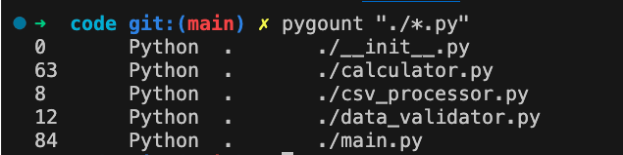
\includegraphics[width=12cm]{images/physicalsloc.png}
    \caption{Physical SLOC calculation using pygount tool}
\end{figure}

\item \textbf{Logical SLOC} \\
The logical SLOC of the METRICSTICS app is calculated manually based on the number of logical statements or instructions in the source code that affect the program's control flow and/or behaviour.
Only the lines of code that contain actual executable operations were counted. This includes conditional statements, loops, actual operational code within functions/methods, such as data processing, calculations, exception handling, input/output operations, and other executed operations

\vspace{12pt}

\begin{table}[!htb]
\centering
\begin{tabular}{|l|l|l|}
\hline
\textbf{Class Name} & \textbf{Physical SLOC} & \textbf{Logical SLOC} \\
\hline
calculator.py           & 63    & 38\\
\hline
csv\_processor.py        & 8     & 3\\
\hline
data\_validator.py       & 11    & 6\\
\hline
main.py                 & 84     & 59\\
\hline
\textbf{Total:}         & 167   & 106\\
\hline
\end{tabular}
\end{table}

\end{enumerate}

\subsection{Qualitative Conclusions}

\begin{enumerate}
    \item A system with a total of 167 physical SLOC implies a smaller size, indicating lower complexity. The reduced size suggests easier maintenance due to its compact nature.
    \item An 106 count of logical Source Lines of Code (SLOC) implies that the software project is relatively small compared to generic systems, potentially featuring a more straightforward and manageable source code. However, it's important to note that relying solely on logical SLOC may not present a complete picture. To gain a more comprehensive understanding of the project, it is crucial to take into account other metrics and factors as well.
    \item The difference between the logical SLOC of 106 and the physical SLOC of 167 is significant and may require further review of the code to confirm whether there are excessive comments, structural elements, or the code can be further optimized to increase the competition of the code. strength and maintenance.
\end{enumerate}

